\documentclass[12pt]{article}
%\usepackage[cp1251]{inputenc}
\usepackage[utf8]{inputenc}
\usepackage[T2A,T1]{fontenc} 
\usepackage[bulgarian]{babel}
\usepackage{amssymb,amsmath,amsfonts,amstext,amscd,latexsym}
\usepackage{graphicx}
\usepackage{amsmath}
\usepackage{amsthm}
\newtheorem*{lemma}{Лема}
\newtheorem*{theorem}{Теорема}
\newtheorem*{definition}{Дефиниция}
\usepackage[shortlabels]{enumitem}
\usepackage[colorinlistoftodos]{todonotes}
\usepackage{braket}
\usepackage{systeme}
\usepackage{hyperref}
\usepackage{titling}
\usepackage{xcolor}
\hypersetup{
	colorlinks   = true, %Colours links instead of boxes
	urlcolor     = blue, %Colour for external hyperlinks
	linkcolor    = blue, %Colour of internal links
	citecolor   = blue %Colour of citations
}
\usepackage[superscript]{cite}
\usepackage[font={small,it}]{caption}
\usepackage[geometry]{ifsym}
\usepackage{listings}
\usepackage{float}
\usepackage{color}
\usepackage{svg}
\usepackage{tabularx}

\begin{document}
	\begin{titlepage}	
		\begin{center}
		
		\newcommand{\HRule}{\rule{\linewidth}{0.5mm}} % Defines a new command for the horizontal lines, change thickness here
		
		
		\textsc{\LARGE Софийски университет }\\[0.3cm]
		\textsc{\LARGE "Св. Климент Охридски" }\\[0.3cm]
		\textsc{\Large Факултет по математика и информатика }\\[0.5cm]
		\textsc{\Large Представяне и моделиране на знания }\\[0.1cm]
		%\fontsize{size}{baselineskip}
		
		
		\vspace{15pt}\centering спец. Изкуствен интелект, I курс, летен семестър \newline учебна година 2025/2026
		\vspace{30pt}
		
		\begin{minipage}{0.4\textwidth}
			\begin{flushleft}\large
				\emph{Изготвил:} \\
				Кристиян Симов \\ 
				фак. номер 4MI3400288 \\ 
				група: 1 %Попълнете вашето име, факултетен номер и група.
			\end{flushleft}
		\end{minipage}
		~
		%\begin{flushleft}
		\begin{minipage}{0.4\textwidth}
			\begin{flushright}
				\large
				\emph{Дата:}\\
				22. 01. 2026 г. % Попълнете датата на предаване
				\\София 
			\end{flushright}
		\end{minipage}\\[1cm]
		%\end{flushleft}
		\bigskip
		{\large \textbf{Онтология на надразред динозаври}}\\
		{\large \textbf{(система от първи тип)}}\\[1cm] 
		%\includegraphics{rsz_sofia_university_logo.png}\\[1cm] 
		\includegraphics{logo_su_no_text.png}\\[1cm]
		\vfill % Fill the rest of the page with whitespace
		\end{center}
	\end{titlepage}
	
	
	\tableofcontents
	
	\newpage
	
	\section{Въведение}\label{sec:introduction}
	
	Динозаврите (Dinosauria) са надразред Животни (царство Animalia) от клас Влечуги (Sauropsida). В продължение на повече от 160 млн. години, започвайки от късния триас преди около 230 млн. години, те са най-широко разпространените сухоземни гръбначни животни на Земята. В края на периода креда, преди около 65 млн. години, динозаврите претърпяват катастрофално масово измиране, от което оцеляват само някои птици, също част от групата на динозаврите, обособила се през юра.\newline\newline Динозаврите са много разнородна група животни, а птиците, с повече от 9 хил. вида са най-разнородната група съвременни гръбначни след бодлоперките. Освен птиците, палеонтолозите разграничават над 500 рода и 1000 вида динозаври. Динозаврите присъстват на всички континенти, както като съществуващи днес видове птици, така и като фосилни находки. Част от динозаврите са растителноядни, а други – хищни, някои се придвижват на два крака, други – на четири, а трети могат да ходят и на два, и на четири крака. Много видове са развили сложни скелетни форми, като брони, рогове или черупки, а повечето изграждат гнезда, в които снасят яйцата си. Макар и известни с големите размери на някои видове, повечето динозаври имат човешки ръст или са по-дребни.
	
	
	\newpage
	
	
	\section{Цел на проекта}\label{sec:goals}
	
	Настоящия проект има за цел да предостави система, която би могла да бъде полезна на учените палеонтолози за специфициране и класифициране на открити от вкаменелости екземпляри (специмени от фосилни находки), изграждане на концепции и хипотези свързани с тях, както и изпълняване на сложни заявки, които биха могли да помогнат за извършване на ключови наблюдения и изграждане на научни теории.\newline\newline По същество това става посредством база от знания, представляваща онтология, чийто граф е разделен умишлено в две основни обособени свързани компоненти. Те отделят концепцията за таксономия, абстрактно знание от сферата на еволюционната биология, където е трудно да има сигурност на изводите, от концепцията за екземпляр (специмен) - реална физическа фосилна находка от сферата на геологията. \newline\newline Така първия слой на онтологията, свързан изцяло с концепцията за специмен позволява на ученият да дефинира параметрите (измерванията) му и свърже дадената реална находка с доказателствата по нея, научни статии, в които това е описано, както и хипотези базирани на изброените, които имат определено ниво на достоверност и приемане в научните следи. Той би могъл до посочи за даден специмен считания за него от науката до момента клас от таксономията ръчно, тъй като тя е отделена във втория слой на онтологията, който моделира точно и детайлно, основаващо се на последни филогенетични проучвания, таксономията на надразред динозаври. Това включва всички разреди, семейства, трибове и родове, което има за цел да позволи генерализации и автоматични изводи/класификации при дефиниране на концепции базиращи се върху тях.\newline\newline Например може да бъде дефинирано какво е хищник, съответно хищен теропод, какво е фамилия на масивни тревопасни, какво е възрастен специмен, както и какво е специмен с доказателства за патологии, такъв от определена ера и същевременно участващ в дадена научна хипотеза, свързана с хищническо или друго поведение.
	
	% trim=left bottom right top
	%\begin{figure}[h]
	%	\centering
	%	\includegraphics[width=1.6\textwidth, trim=30mm 8cm 0mm 1cm, clip]{dinosauria.pdf}
	%	\caption{Модел на разред динозаври}
	%	\label{fig:dinosauria}
	%\end{figure}
	
	
	\newpage
	
	\section{База от знания - елементи на онтологията}\label{sec:knowledgebase}
	Както вече беше упоменато, базата от знания и съответно елементите на онтологията се поделят в две основни части. От една страна имаме имаме моделирана йерархия от концепции, представляваща пълната и точна таксономия на надразред динозаври, която предстои да бъде описана наблягайки на основните концепции, като пълната такава, разработена на база проучване научни статии може да бъде видяна в съпътстващия документация файл dinosauria.svg от архива. На другият слой от онтологията имаме елементите от слоя свързан с физическите находки (специмените), които предоставят средства за изчерпателно описване на даден индивид посредством множество свойства от този домейн, както и помощни концепции с техните специфични свойства.
	
	\subsection{Слой надразред динозаври (таксономия)}
	\subsubsection{Класове}
		\noindent\begin{tabularx}{\textwidth}{|X|}
			\hline
			\textbf{Taxon} $\sqsubseteq$ owl:Thing \\
			\hline
			\textbf{Animalia} $\sqsubseteq$ Taxon \\
			\hline
			\textbf{Dinosauria} $\sqsubseteq$ Animalia \\
			\hline
			\textbf{Ornithischia} $\sqsubseteq$ Dinosauria \\
			\hline
			\textbf{Saurischia} $\sqsubseteq$ Dinosauria \\
			\hline
			\textbf{...} $\sqsubseteq$ ... \\
			\hline
			\textbf{Genasauria} $\sqsubseteq$ ... \\
			\hline
			\textbf{Thyreophora} $\sqsubseteq$ Genasauria \\
			\hline
			\textbf{Neornithischia} $\sqsubseteq$ Genasauria \\
			\hline
			\textbf{...} $\sqsubseteq$ ... \\
			\hline
			\textbf{Eurypoda} $\sqsubseteq$ ... \\
			\hline
			\textbf{Stegosauria} $\sqsubseteq$ Eurypoda \\
			\hline
			\textbf{Ankylosauria} $\sqsubseteq$ Eurypoda \\
			\hline
			\textbf{...} $\sqsubseteq$ ... \\
			\hline
			\textbf{Cerapoda} $\sqsubseteq$ ... \\
			\hline
			\textbf{Marginocephalia} $\sqsubseteq$ Cerapoda \\
			\hline
			\textbf{Ornithopoda} $\sqsubseteq$ Cerapoda \\
			\hline
			\textbf{...} $\sqsubseteq$ ... \\
			\hline
			\textbf{Styracosterna} $\sqsubseteq$ ... \\
			\hline
			\textbf{Hadrosauriformes} $\sqsubseteq$ Styracosterna \\
			\hline
			\textbf{Ceratopsia} $\sqsubseteq$ Marginocephalia \\
			\hline
			\textbf{...} $\sqsubseteq$ ... \\
			\hline
			\textbf{Eusaurischia} $\sqsubseteq$ ... \\
			\hline
			\textbf{Sauropodomorpha} $\sqsubseteq$ Eusaurischia \\
			\hline
			\textbf{Theropoda} $\sqsubseteq$ Eusaurischia \\
			\hline
			\textbf{...} $\sqsubseteq$ ... \\
			\hline
			\textbf{MassapodaMassospondylidaeSauropodiformes} $\sqsubseteq$ ... \\
			\hline
			\textbf{Sauropodiformes} $\sqsubseteq$ MassapodaMassospondylidaeSauropodiformes \\
			\hline
			\textbf{...} $\sqsubseteq$ ... \\
			\hline
			\textbf{Macronaria} $\sqsubseteq$ ... \\
			\hline
			\textbf{Titanosauriformes} $\sqsubseteq$ Macronaria \\
			\hline
			\textbf{...} $\sqsubseteq$ ... \\
			\hline
			\textbf{Averostra} $\sqsubseteq$ ... \\
			\hline
			\textbf{Ceratosauria} $\sqsubseteq$ Averostra \\
			\hline
		\end{tabularx}
		\newpage
		\noindent\begin{tabularx}{\textwidth}{|X|}
			\hline
			\textbf{...} $\sqsubseteq$ ... \\
			\hline
			\textbf{Tetanurae} $\sqsubseteq$ ... \\
			\hline
			\textbf{Carnosauria} $\sqsubseteq$ Tetanurae \\
			\hline
			\textbf{Coelurosauria} $\sqsubseteq$ Tetanurae \\
			\hline
			\textbf{...} $\sqsubseteq$ ... \\
			\hline
			\textbf{Tyrannoraptora} $\sqsubseteq$ ... \\
			\hline
			\textbf{Maniraptoromorpha} $\sqsubseteq$ Tyrannoraptora \\
			\hline
			\textbf{...} $\sqsubseteq$ ... \\
			\hline
			\textbf{ManiraptoraPennaraptora} $\sqsubseteq$ ... \\
			\hline
			\textbf{Pennaraptora} $\sqsubseteq$ ManiraptoraPennaraptora \\
			\hline
			\textbf{Paraves} $\sqsubseteq$ Pennaraptora \\
			\hline
			\textbf{Averaptora} $\sqsubseteq$ Paraves \\
			\hline
			\textbf{...} $\sqsubseteq$ ... \\
			\hline
			\textbf{PygostyliaOrnithothoraces} $\sqsubseteq$ ... \\
			\hline
			\textbf{Ornithothoraces} $\sqsubseteq$ PygostyliaOrnithothoraces \\
			\hline
			\textbf{...} $\sqsubseteq$ ... \\
			\hline
			\textbf{Euornithes} $\sqsubseteq$ ... \\
			\hline
			\textbf{Ornithurae} $\sqsubseteq$ Euornithes \\
			\hline
			\textbf{...} $\sqsubseteq$ ... \\
			\hline
			\textbf{OrnithuraeIchthyornithesVegaviidaeAves} $\sqsubseteq$ ... \\
			\hline
			\textbf{Aves} $\sqsubseteq$ OrnithuraeIchthyornithesVegaviidaeAves \\
			\hline
		\end{tabularx}
		\newline
		\newline
		Дотук описахме опростената таксономия, която стига до днешните птици (Aves) и не включва родове. Сега ще включим някои от по-известните трибове и подсемейства, за да опишем няколко вида (концепти листа):
		\newline
		\newline
		\noindent\begin{tabularx}{\textwidth}{|X|}
			\hline
			\textbf{...} $\sqsubseteq$ ... \\
			\hline
			\textbf{Stegosaurinae} $\sqsubseteq$ ... \\
			\hline
			\textbf{Stegosaurus} $\sqsubseteq$ Stegosaurinae \\
			\hline
			\textbf{...} $\sqsubseteq$ ... \\
			\hline
			\textbf{Ankylosaurinae} $\sqsubseteq$ ... \\
			\hline
			\textbf{Ankylosaurus} $\sqsubseteq$ Ankylosaurinae \\
			\hline
			\textbf{...} $\sqsubseteq$ ... \\
			\hline
			\textbf{Parasaurolophini} $\sqsubseteq$ ... \\
			\hline
			\textbf{Parasaurolophus} $\sqsubseteq$ Parasaurolophini \\
			\hline
			\textbf{...} $\sqsubseteq$ ... \\
			\hline
		\end{tabularx}
		\newpage
		\noindent\begin{tabularx}{\textwidth}{|X|}
			\hline
			\textbf{Triceratopsini} $\sqsubseteq$ ... \\
			\hline
			\textbf{Triceratops} $\sqsubseteq$ Triceratopsini \\
			\hline
			\textbf{...} $\sqsubseteq$ ... \\
			\hline
			\textbf{...} $\sqsubseteq$ ... \\
			\hline
			\textbf{Diplodocinae} $\sqsubseteq$ ... \\
			\hline
			\textbf{Diplodocus} $\sqsubseteq$ Diplodocinae \\
			\hline
			\textbf{...} $\sqsubseteq$ ... \\
			\hline
			\textbf{Brachiosauridae} $\sqsubseteq$ ... \\
			\hline
			\textbf{Brachiosaurus} $\sqsubseteq$ Brachiosauridae \\
			\hline
			\textbf{...} $\sqsubseteq$ ... \\
			\hline
			\textbf{Furileusauria} $\sqsubseteq$ ... \\
			\hline
			\textbf{Carnotaurus} $\sqsubseteq$ Furileusauria \\
			\hline
			\textbf{...} $\sqsubseteq$ ... \\
			\hline
			\textbf{Spinosaurini} $\sqsubseteq$ ... \\
			\hline
			\textbf{Spinosaurus} $\sqsubseteq$ Spinosaurini \\
			\hline
			\textbf{...} $\sqsubseteq$ ... \\
			\hline
			\textbf{Allosauridae} $\sqsubseteq$ ... \\
			\hline
			\textbf{Allosaurus} $\sqsubseteq$ Allosauridae \\
			\hline
			\textbf{...} $\sqsubseteq$ ... \\
			\hline
			\textbf{Tyrannosaurini} $\sqsubseteq$ ... \\
			\hline
			\textbf{Tyrannosaurus} $\sqsubseteq$ Tyrannosaurini \\
			\hline
			\textbf{...} $\sqsubseteq$ ... \\
			\hline
			\textbf{Therizinosauridae} $\sqsubseteq$ ... \\
			\hline
			\textbf{Therizinosaurus} $\sqsubseteq$ Therizinosauridae \\
			\hline
			\textbf{...} $\sqsubseteq$ ... \\
			\hline
			\textbf{Velociraptorinae} $\sqsubseteq$ ... \\
			\hline
			\textbf{Deinonychus} $\sqsubseteq$ Velociraptorinae \\
			\hline
		\end{tabularx}
	\subsubsection{Индивиди}
	Описаната преди малко таксономия по дизайн не предполага да бъдат създавани индивиди (екземпляри). Разделението на онтологията предполага това да става в слоят свързан със специмените. В текущия слой обаче е възможно класифициране както и дефиниране на генерални свойства и концепти свързани с йерархичната структура.
	\newpage
	\subsubsection{Свойства}
	\begin{tabular}{ | m{3.8cm} | m{3.8cm}| m{3.8cm} | m{3.8cm} | } 
		\hline
		\textbf{Domain} & \textbf{Property} & \textbf{Range} & \textbf{Characteristics} \\ 
		\hline
		Animalia & HasNaturalPredator & Animalia & ObjectProperty AsymmetricProperty IrreflexiveProperty \\ 
		\hline
		Animalia & IsNaturalPredatorOf & Animalia & ObjectProperty AsymmetricProperty IrreflexiveProperty inverseOf HasNaturalPredator \\  
		\hline
		Animalia & PossiblyPreyedOn & Animalia & ObjectProperty weaker semantics \\ 
		\hline
	\end{tabular}
	
	\subsubsection{Концепти (неатомарни)}
	
	\noindent\begin{tabularx}{\textwidth}{|X|}
		\hline
		\textbf{Carnivore} $\doteq$ [AND Animalia [EXISTS 1 :IsNaturalPredatorOf]] \\
		\hline
		\textbf{ApexPredator} $\doteq$ [AND Carnivore [EXACTLY 0 :HasNaturalPredator]] \\
		\hline
		\textbf{TheropodCarnivore} $\doteq$ [AND Theropoda Carnivore]] \\
		\hline
		\textbf{LargeBodiedHerbivorousLineage} $\doteq$ \newline \{Hadrosauriformes\} $\sqcup$ \{Ceratopsidae\}  $\sqcup$ \{Sauropodiformes\} \\
		\hline
	\end{tabularx}
	
	
	\newpage
	
	\subsection{Слой специмени (физически находки)}
	\subsubsection{Класове}
	\noindent\begin{tabularx}{\textwidth}{|X|}
		\hline
		\textbf{Specimen} $\sqsubseteq$ owl:Thing \\
		\hline
		\textbf{Place} $\sqsubseteq$ owl:Thing \\
		\hline
		\textbf{Formation} $\sqsubseteq$ Place \\
		\hline
		\textbf{Site} $\sqsubseteq$ Place \\
		\hline
		\textbf{Museum} $\sqsubseteq$ Place \\
		\hline
		\textbf{Location} $\sqsubseteq$ owl:Thing \\
		\hline
		\textbf{Person} $\sqsubseteq$ owl:Thing \\
		\hline
		\textbf{Discoverer} $\sqsubseteq$ Person \\
		\hline
		\textbf{AnatomicalElement} $\sqsubseteq$ owl:Thing \\
		\hline
		\textbf{Femur} $\sqsubseteq$ AnatomicalElement \\
		\hline
		\textbf{Skull} $\sqsubseteq$ AnatomicalElement \\
		\hline
		\textbf{TaxonConcept} $\sqsubseteq$ owl:Thing \\
		\hline
		\textbf{AssertiveEntity} $\sqsubseteq$ owl:Thing \\
		\hline
		\textbf{Evidence} $\sqsubseteq$ AssertiveEntity \\
		\hline
		\textbf{BiteMarkEvidence} $\sqsubseteq$ Evidence \\
		\hline
		\textbf{PathologyEvidence} $\sqsubseteq$ Evidence \\
		\hline
		\textbf{Hypothesis} $\sqsubseteq$ AssertiveEntity \\
		\hline
		\textbf{PredationHypothesis} $\sqsubseteq$ Hypothesis \\
		\hline
		\textbf{ConfidenceLevel} $\sqsubseteq$ owl:Thing \\
		\hline
		\textbf{Publication} $\sqsubseteq$ owl:Thing \\
		\hline
		\textbf{Eon} $\sqsubseteq$ owl:Thing \\
		\hline
		\textbf{Phanerozoic} $\sqsubseteq$ Eon \\
		\hline
		\textbf{Era} $\sqsubseteq$ Eon \\
		\hline
		\textbf{Mesozoic} $\sqsubseteq$ Era \\
		\hline
		\textbf{Period} $\sqsubseteq$ Era \\
		\hline
		\textbf{Triassic} $\sqsubseteq$ Period \\
		\hline
		\textbf{Jurassic} $\sqsubseteq$ Period \\
		\hline
		\textbf{Cretaceous} $\sqsubseteq$ Period \\
		\hline
		\textbf{Age} $\sqsubseteq$ Period \\
		\hline
		\textbf{Induan} $\sqsubseteq$ Age \\
		\hline
		\textbf{...} $\sqsubseteq$ ... \\
		\hline
		\textbf{Hettangian} $\sqsubseteq$ Age \\
		\hline
		\textbf{...} $\sqsubseteq$ ... \\
		\hline
		\textbf{Maastrichtian} $\sqsubseteq$ Age \\
		\hline
	\end{tabularx}
	\newpage
	\subsubsection{Индивиди}
	\noindent\begin{tabularx}{\textwidth}{|X|}
		\hline
		\textbf{HighConfidence} $\longrightarrow$ ConfidenceLevel \\
		\hline
		\textbf{MediumConfidence} $\longrightarrow$ ConfidenceLevel \\
		\hline
		\textbf{LowConfidence} $\longrightarrow$ ConfidenceLevel \\
		\hline
		\textbf{LateMaastrichtian} $\longrightarrow$ Maastrichtian \\
		\hline
		\textbf{CrowsnestPass\_Alberta\_Canada} $\longrightarrow$ Location \\
		\hline
		\textbf{Washington\_DC\_USA} $\longrightarrow$ Location \\
		\hline
		\textbf{Drumheller\_Alberta} $\longrightarrow$ Location  \\
		\hline
		\textbf{Wyoming\_USA} $\longrightarrow$ Location \\
		\hline
		\textbf{CrowsnestPass\_ExcavationSite} $\longrightarrow$ [AND Site [FILLS :HasLocation CrowsnestPass\_Alberta\_Canada]] \\
		\hline
		\textbf{HatcherDiscoverySite} $\longrightarrow$ [AND Site [FILLS :HasLocation Wyoming\_USA]] \\
		\hline
		\textbf{WillowCreekFormation} $\longrightarrow$ [AND Formation [FILLS :HasLocation CrowsnestPass\_Alberta\_Canada]] \\
		\hline
		\textbf{LanceFormation} $\longrightarrow$ [AND Formation [FILLS :HasLocation  Wyoming\_USA]] \\
		\hline
		\textbf{RoyalTyrrellMuseum} $\longrightarrow$ [AND Museum [FILLS :HasLocation Drumheller\_Alberta]] \\
		\hline
		\textbf{Smithsonian\_NMNH} $\longrightarrow$ [AND Museum [FILLS :HasLocation Washington\_DC\_USA]] \\
		\hline
		\textbf{JeffBaker} $\longrightarrow$ Discoverer \\
		\hline
		\textbf{JohnBellHatcher} $\longrightarrow$ Discoverer \\
		\hline
		\textbf{TyrannosaurusConcept} $\longrightarrow$ [AND TaxonConcept [FILLS :refers\_to\_named\_taxon Tyrannosaurus]] \\
		\hline
		\textbf{TriceratopsConcept} $\longrightarrow$ [AND TaxonConcept [FILLS :refers\_to\_named\_taxon Triceratops]] \\
		\hline
		
		\textbf{Horner2009} $\longrightarrow$ [AND Publication [FILLS :has\_DOI "10.1371/journal.pone.0007288"] [FILLS :publication\_year 2009] [FILLS :hasAuthor "Horner"] [FILLS :hasAuthor "Salisbury"] [FILLS :hasAuthor "Wolff"]] \\
		\hline
		\textbf{Smith2012} $\longrightarrow$ [AND Publication [FILLS :has\_DOI "10.1234/paleo.2012.001"] [FILLS :publication\_year 2012] [FILLS :hasAuthor "Smith"]] \\
		\hline
		\textbf{Smithsonian\_HatcherHistory\_2018} $\longrightarrow$ Publication \\
		\hline
	\end{tabularx}
	\newpage
	\noindent\begin{tabularx}{\textwidth}{|X|}
		\hline
		\textbf{HatcherBiteMarks} $\longrightarrow$ [AND BiteMarkEvidence [FILLS :InferredFromTaxon TyrannosaurusConcept] [FILLS :evidence\_notes "Exhibit designs suggest possible Tyrannosaurus feeding..."]] \\
		\hline
		\textbf{HatcherPyriteDisease} $\longrightarrow$ [AND PathologyEvidence [FILLS :HasConfidenceLevel HighConfidence] [FILLS :evidence\_notes "Evidence of pyrite disease causing internal bone breakage."] [FILLS :HasCitation Smithsonian\_HatcherHistory\_2018]] \\
		\hline
		\textbf{BlackBeautyCranialPathology} $\longrightarrow$ [AND PathologyEvidence [FILLS :HasConfidenceLevel HighConfidence] [FILLS :evidence\_notes "Cranial bone lesions interpreted as evidence of parasitic infection."] [FILLS :HasCitation Horner2009]] \\
		\hline
		\textbf{TyrannosaurusPreyedOnTriceratops} $\longrightarrow$ [AND PredationHypothesis [FILLS :InvolvesPredator TyrannosaurusConcept] [FILLS :InvolvesPrey TriceratopsConcept] [FILLS :SupportedBy HatcherBiteMarks] [FILLS :HasConfidenceLevel MediumConfidence] [FILLS :HasCitation Smith2012]] \\
		\hline
		\textbf{BlackBeauty} $\longrightarrow$ [AND Specimen [FILLS :number "RTMP 81.6.1"] [FILLS :from\_million\_years\_ago 69] [FILLS :until\_million\_years\_ago HatcherBiteMarks 66] [FILLS :completeness 0.85] [FILLS :year\_collected 1980] [FILLS :ExcavatedFromSite CrowsnestPass\_ExcavationSite] [FILLS :FoundInFormation WillowCreekFormation] [FILLS :CuratedAt RoyalTyrrellMuseum] [FILLS :DiscoveredBy JeffBaker] [FILLS :growthStage "adult"] [FILLS :DatedTo LateMaastrichtian] [FILLS :HasEvidence BlackBeautyCranialPathology] [FILLS :DescribedIn Horner2009] [FILLS :notes "Nickname refers to dark coloration caused by mineralization during fossilization."]] $\sqcup$ Tyrannosaurus \\
		\hline
		\textbf{Hatcher} $\longrightarrow$ [AND Specimen [FILLS :number "USNM \#\#\#\#"] [FILLS :from\_million\_years\_ago 68] [FILLS :until\_million\_years\_ago HatcherBiteMarks 66] [FILLS :completeness 1.0] [FILLS :year\_collected 1888] [FILLS :ExcavatedFromSite HatcherDiscoverySite] [FILLS :FoundInFormation LanceFormation] [FILLS :CuratedAt Smithsonian\_NMNH] [FILLS :DiscoveredBy JohnBellHatcher] [FILLS :growthStage "adult"] [FILLS :DatedTo LateMaastrichtian] [FILLS :HasEvidence HatcherBiteMarks] [FILLS :HasEvidence HatcherPyriteDisease] [FILLS :DescribedIn Smithsonian\_HatcherHistory\_2018] [FILLS :notes "First Triceratops specimen put on exhibit in 1905, pieced together from multiple individuals.]] $\sqcup$ Triceratops \\
		\hline
	\end{tabularx}
	\newpage
	\subsubsection{Свойства}
	\begin{tabular}{ | m{3cm} | m{4.5cm}| m{3.5cm} | m{3.8cm} | } 
		\hline
		\textbf{Domain} & \textbf{Property} & \textbf{Range} & \textbf{Characteristics} \\
		\hline
		Specimen & number & xsd:string & DataProperty FunctionalProperty \\ 
		\hline
		Specimen & notes & xsd:string & DataProperty \\ 
		\hline
		Specimen & year\_collected & xsd:int & DataProperty FunctionalProperty \\ 
		\hline
		Specimen & from\_million\_years\_ago & xsd:float & DataProperty FunctionalProperty \\ 
		\hline
		Specimen & until\_million\_years\_ago & xsd:float & DataProperty FunctionalProperty \\ 
		\hline
		Specimen & completeness & xsd:float & DataProperty FunctionalProperty \\ 
		\hline
		Specimen & estimated\_mass & xsd:float & DataProperty FunctionalProperty \\ 
		\hline
		Specimen & DatedTo & Period & ObjectProperty \\ 
		\hline
		Specimen & FoundInFormation & Formation & ObjectProperty \\ 
		\hline
		Specimen & ExcavatedFromSite & Site & ObjectProperty \\ 
		\hline
		Specimen & CuratedAt & Museum & ObjectProperty \\ 
		\hline
		Specimen & DiscoveredBy & Discoverer & ObjectProperty \\ 
		\hline
		Specimen & DescribedIn & Publication & ObjectProperty \\ 
		\hline
		Specimen & HasEvidence & Evidence & ObjectProperty \\ 
		\hline
		Specimen & hasPreservedElement & AnatomicalElement & ObjectProperty \\ 
		\hline
		Specimen & HasBiteMarksFrom & Specimen & ObjectProperty \\ 
		\hline
	\end{tabular}
	\newpage
	\noindent\begin{tabular}{ | m{3.6cm} | m{4.5cm}| m{3.5cm} | m{3.8cm} | } 
		\hline
		\textbf{Domain} & \textbf{Property} & \textbf{Range} & \textbf{Characteristics} \\
		\hline
		Period & IncludesDatedSpecimen & Specimen & ObjectProperty inverseOf DatedTo \\ 
		\hline
		Publication & has\_DOI & xsd:string & DataProperty FunctionalProperty \\ 
		\hline
		Publication & publication\_year & xsd:integer & DataProperty FunctionalProperty \\  
		\hline
		Publication & hasAuthor & xsd:string & DataProperty \\ 
		\hline
		Hypothesis & SupportedBy & Evidence & ObjectProperty \\ 
		\hline
		AssertiveEntity & HasCitation & Publication & ObjectProperty \\ 
		\hline
		AssertiveEntity & HasConfidenceLevel & ConfidenceLevel & ObjectProperty \\ 
		\hline
		TaxonConcept & refers\_to\_named\_taxon & xsd:string & DataProperty FunctionalProperty \\ 
		\hline
		TaxonConcept & has\_taxon\_identifier & xsd:string & DataProperty FunctionalProperty \\ 
		\hline
		Place & HasLocation & Location & ObjectProperty \\ 
		\hline
		Evidence & interpretation\_confidence & xsd:float & DataProperty FunctionalProperty \\ 
		\hline
		Evidence & evidence\_notes & xsd:string & DataProperty \\ 
		\hline
		Evidence & ObservedOn & Specimen & ObjectProperty inverseOf HasEvidence \\ 
		\hline
		Evidence & InferredFromTaxon & TaxonConcept & ObjectProperty \\ 
		\hline
		PredationHypothesis & InvolvesPredator & TaxonConcept & ObjectProperty \\ 
		\hline
		PredationHypothesis & InvolvesPrey & TaxonConcept & ObjectProperty \\ 
		\hline
	\end{tabular}
	\newpage
	
	\subsubsection{Концепти (неатомарни)}
	
	\noindent\begin{tabularx}{\textwidth}{|X|}
		\hline
		\textbf{AdultSpecimen} $\doteq$ [AND Specimen [FILLS :growthStage "adult"]] \\
		\hline
		\textbf{MaastrichtianSpecimen} $\doteq$ [AND Specimen [FILLS :DatedTo Maastrichtian]] \\
		\hline
		\textbf{PathologicalSpecimen} $\doteq$ [AND Specimen [FILLS :HasEvidence PathologyEvidence] \\
		\hline
		\textbf{PathologicalTyrannosaurusSpecimen} $\doteq$ [AND PathologicalSpecimen Tyrannosaurus] \\
		\hline
		\textbf{PathologicalCeratopsianSpecimen} $\doteq$ [AND PathologicalSpecimen Ceratopsidae] \\
		\hline
		\textbf{EvidenceBasedHypothesis} $\doteq$ [AND Hypothesis [FILLS :SupportedBy Evidence] \\
		\hline
		\textbf{PathologySupportedHypothesis} $\doteq$ [AND Hypothesis [FILLS :SupportedBy PathologyEvidence] \\
		\hline
		\textbf{MaastrichtianPathologicalCeratopsianBiteMarkBasedPredation\newline Hypothesis} $\doteq$ \newline [AND PredationHypothesis [FILLS :SupportedBy [AND BiteMarkEvidence [FILLS :ObservedOn [AND MaastrichtianSpecimen PathologicalCeratopsianSpecimen]]]]]\\
		\hline
	\end{tabularx}
	
	
	\newpage
	
	\section{Примери за извършване на логически изводи}\label{sec:inference}
	\subsection{Изводи от вида KB $\vDash$ (D $\sqsubseteq$ E) }
	\subsubsection{KB $\vDash$ (ApexPredator $\sqsubseteq$ Carnivore)}
	\textbf{Carnivore} $\doteq$ [AND Animalia [EXISTS 1 :IsNaturalPredatorOf]]
	\newline
	\textbf{ApexPredator} $\doteq$ [AND \textcolor{green}{Carnivore} [EXACTLY 0 :HasNaturalPredator]]
	\subsubsection{KB $\vDash$ (PathologySupportedHypothesis $\sqsubseteq$ EvidenceBasedHypothesis)}
	\textbf{EvidenceBasedHypothesis} $\doteq$ [AND \textcolor{green}{Hypothesis} [FILLS :SupportedBy \textcolor{green}{Evidence}]
	\newline
	\textbf{PathologyEvidence} $\sqsubseteq$ \textcolor{green}{Evidence}
	\newline
	\textbf{PathologySupportedHypothesis} $\doteq$ [AND \textcolor{green}{Hypothesis} [FILLS :SupportedBy PathologyEvidence]
	\subsubsection{KB $\vDash$ (Maastrichtian...BiteMarkBasedPredationHypothesis $\sqsubseteq$ EvidenceBasedHypothesis)}
	\textbf{EvidenceBasedHypothesis} $\doteq$ [AND \textcolor{green}{Hypothesis} [FILLS :SupportedBy \textcolor{green}{Evidence}]
	\newline
	\textbf{Maastrichtian...BiteMarkBasedPredationHypothesis} $\doteq$ \newline [AND PredationHypothesis [FILLS :SupportedBy [AND BiteMarkEvidence [FILLS :ObservedOn [AND MaastrichtianSpecimen PathologicalCeratopsianSpecimen]]]]]
	\newline
	\textbf{Maastrichtian...BiteMarkBasedPredationHypothesis} $\sqsubseteq$ PredationHypothesis $\sqsubseteq$ \textcolor{green}{Hypothesis}
	\newline
	\textbf{BiteMarkEvidence} $\sqsubseteq$ \textcolor{green}{Evidence}
	
	\newpage
	\subsection{Изводи от вида KB $\vDash$ (C $\longrightarrow$ E) }
	\subsubsection{KB $\vDash$ (BlackBeauty $\longrightarrow$ MaastrichtianSpecimen)}
	\textbf{BlackBeauty} $\longrightarrow$ [AND \textcolor{green}{Specimen} [FILLS :number "RTMP 81.6.1"] ... [FILLS :growthStage "adult"] \textcolor{green}{[FILLS :DatedTo LateMaastrichtian]} [FILLS :HasEvidence BlackBeautyCranialPathology] ... ]
	\newline
	\textbf{LateMaastrichtian} $\longrightarrow$ Maastrichtian
	\newline
	\textbf{MaastrichtianSpecimen} $\doteq$ [AND Specimen [FILLS :DatedTo Maastrichtian]]
	\subsubsection{KB $\vDash$ (BlackBeauty $\longrightarrow$ AdultSpecimen)}
	\textbf{BlackBeauty} $\longrightarrow$ [AND \textcolor{green}{Specimen} [FILLS :number "RTMP 81.6.1"] ... [FILLS :DiscoveredBy JeffBaker] \textcolor{green}{[FILLS :growthStage "adult"]} [FILLS :DatedTo LateMaastrichtian] [FILLS :HasEvidence BlackBeautyCranialPathology] ... ]
	\newline
	\textbf{AdultSpecimen} $\doteq$ [AND Specimen [FILLS :growthStage "adult"]]
	\subsubsection{KB $\vDash$ (BlackBeauty $\longrightarrow$ PathologicalTyrannosaurusSpecimen)}
	\textbf{BlackBeauty} $\longrightarrow$ [AND \textcolor{green}{Specimen} [FILLS :number "RTMP 81.6.1"] ... [FILLS :DatedTo LateMaastrichtian] \textcolor{green}{[FILLS :HasEvidence BlackBeautyCranialPathology]} [FILLS :DescribedIn Horner2009] [FILLS :notes "Nickname refers to dark coloration caused by mineralization during fossilization."]]
	\newline
	\textbf{BlackBeauty} $\longrightarrow$ \textcolor{green}{Tyrannosaurus}
	\newline
	\textbf{BlackBeautyCranialPathology} $\longrightarrow$ [AND \textcolor{green}{PathologyEvidence} ... ] $\sqsubseteq$ PathologyEvidence
	\newline
	\textbf{PathologicalSpecimen} $\doteq$ [AND Specimen [FILLS :HasEvidence PathologyEvidence]
	\newline
	\textbf{PathologicalTyrannosaurusSpecimen} $\doteq$ [AND PathologicalSpecimen Tyrannosaurus]
	
	\subsubsection{KB $\vDash$ (Hatcher $\longrightarrow$ PathologicalCeratopsianSpecimen)}
	\textbf{Hatcher} $\longrightarrow$ [AND \textcolor{green}{Specimen} [FILLS :number "USNM \#\#\#\#"] ... \textcolor{green}{[FILLS :HasEvidence HatcherPyriteDisease]} [FILLS :DescribedIn Smithsonian\_HatcherHistory\_2018] ... ]
		\newline
	\textbf{Hatcher} $\longrightarrow$ Triceratops $\sqsubseteq$ \textcolor{green}{Ceratopsidae}
	\newline
	\textbf{HatcherPyriteDisease} $\longrightarrow$ [AND \textcolor{green}{PathologyEvidence} ... ] $\sqsubseteq$ PathologyEvidence
	\newline
	\textbf{PathologicalSpecimen} $\doteq$ [AND Specimen [FILLS :HasEvidence PathologyEvidence]
	\newline
	\textbf{PathologicalCeratopsianSpecimen} $\doteq$ [AND PathologicalSpecimen Ceratopsidae]
	
	\newpage
	
	\section{Визуализация на онтологията чрез WebVOWL 1.1.7}\label{sec:visualisation}
	
	\begin{figure}[H]
		\centering
		\includegraphics[width=150mm]{figures/dinosaur_onto.png}
		\caption{Онтологията показана отдалече. За по-голям и интерактивен вариант отворете предоставения в архива файл dinosaur\_onto.svg с предпочитан браузър, или заредете също предоставения dinosaur\_onto.owl в онлайн визуализатора WebVOWL 1.1.7 на адрес \href{https://service.tib.eu/webvowl/}{TIB WebVOWL Service}}
	\end{figure}
	\newpage
	\subsection{Слой специмени без филтър на степени}
	\begin{figure}[H]
		\centering
		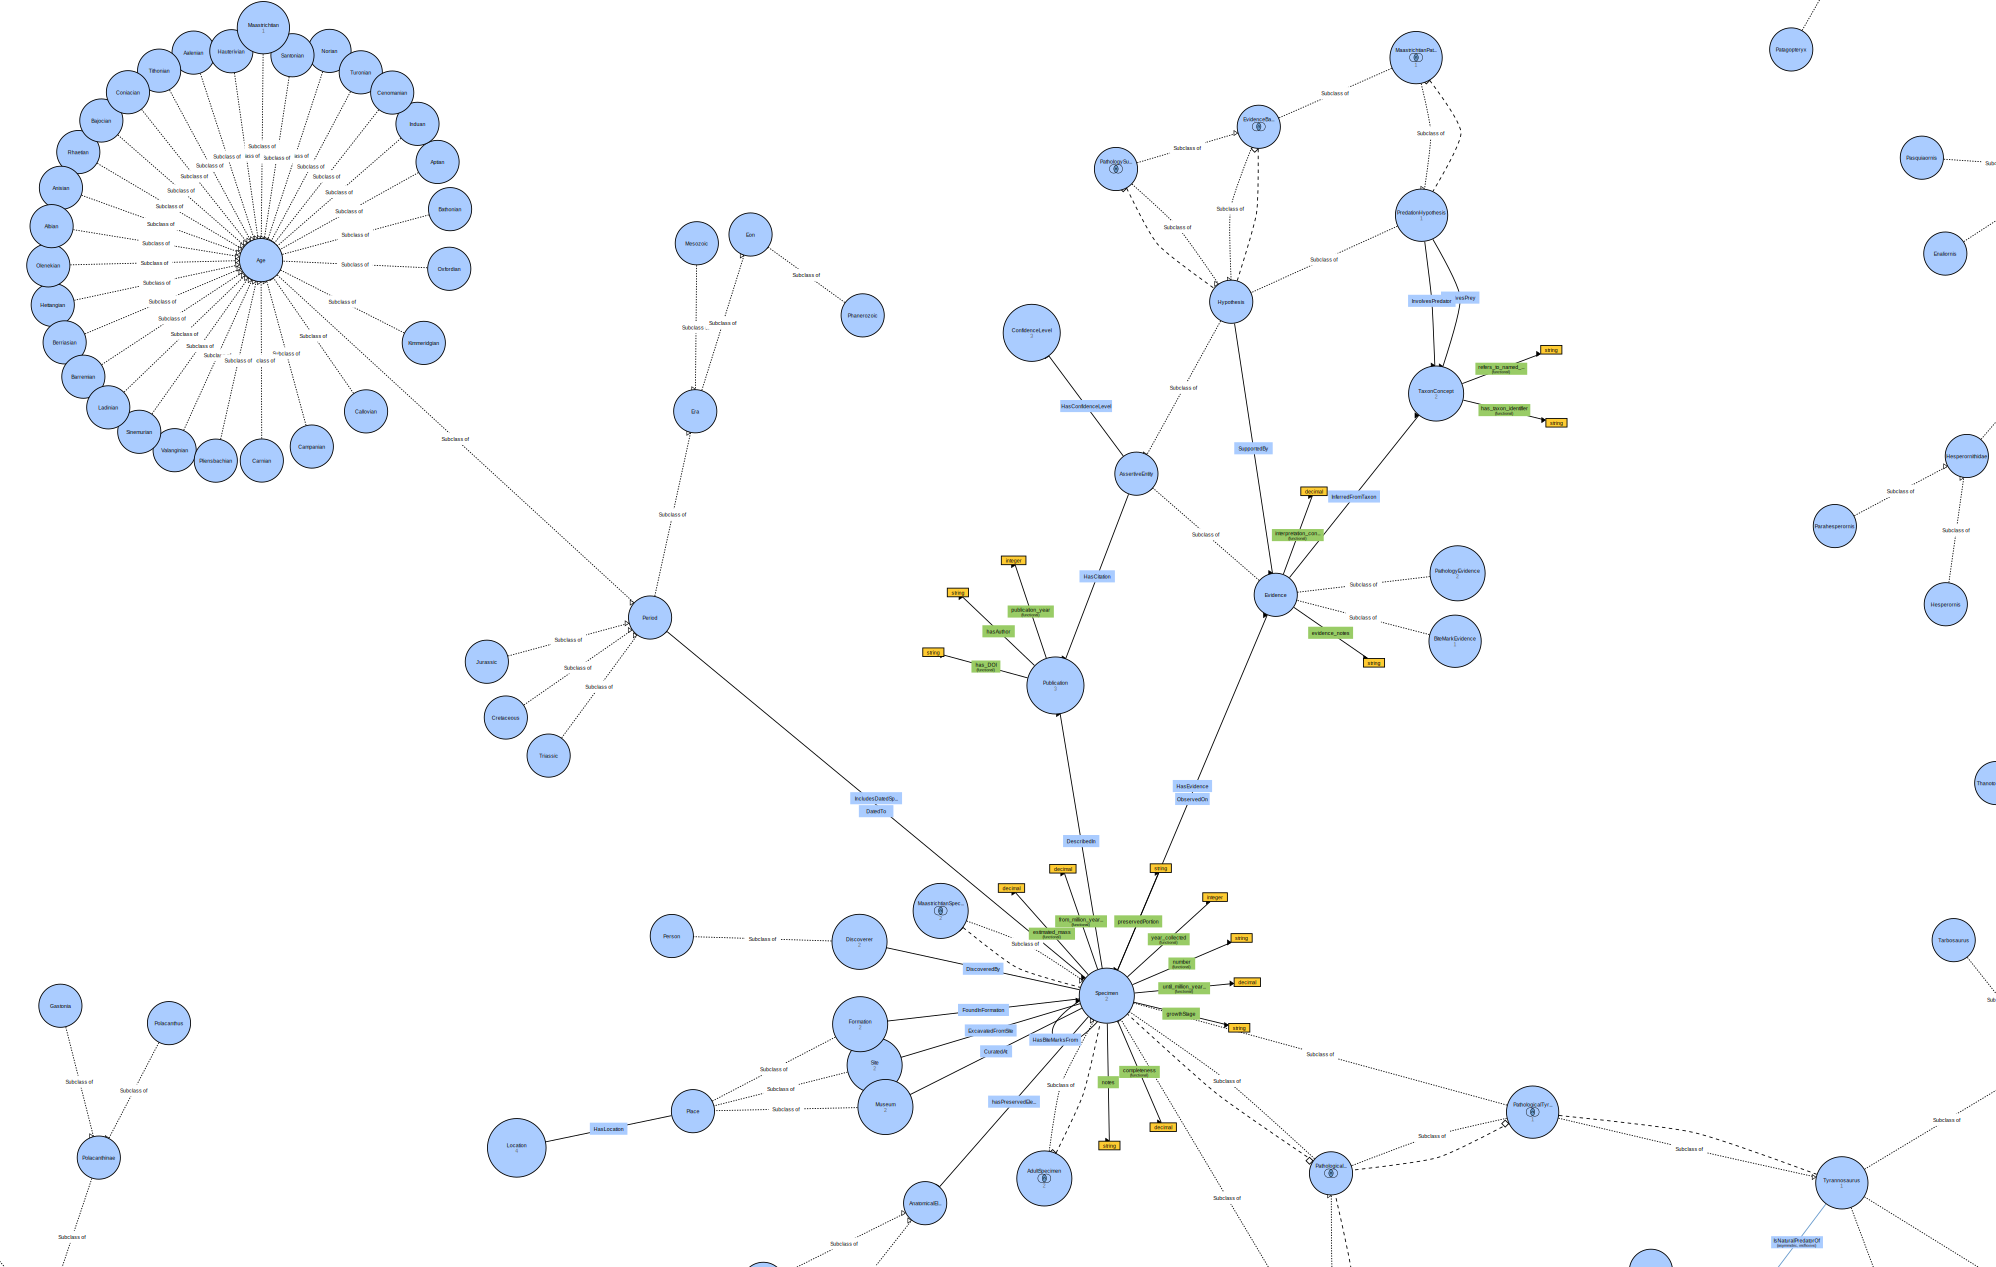
\includegraphics[width=150mm]{figures/specimen_0_degrees_filter.png}
		\caption{Приближение на свързаната компонента (слой) на онтологията с център на тежестта концепция за специмен. За по-голям и интерактивен вариант отворете предоставения в архива файл specimen\_0\_degrees\_filter.svg с предпочитан от вас браузър.}
	\end{figure}
	\newpage
	\subsection{Слой надразред динозаври с филтър на степени}
	\begin{figure}[H]
		\centering
		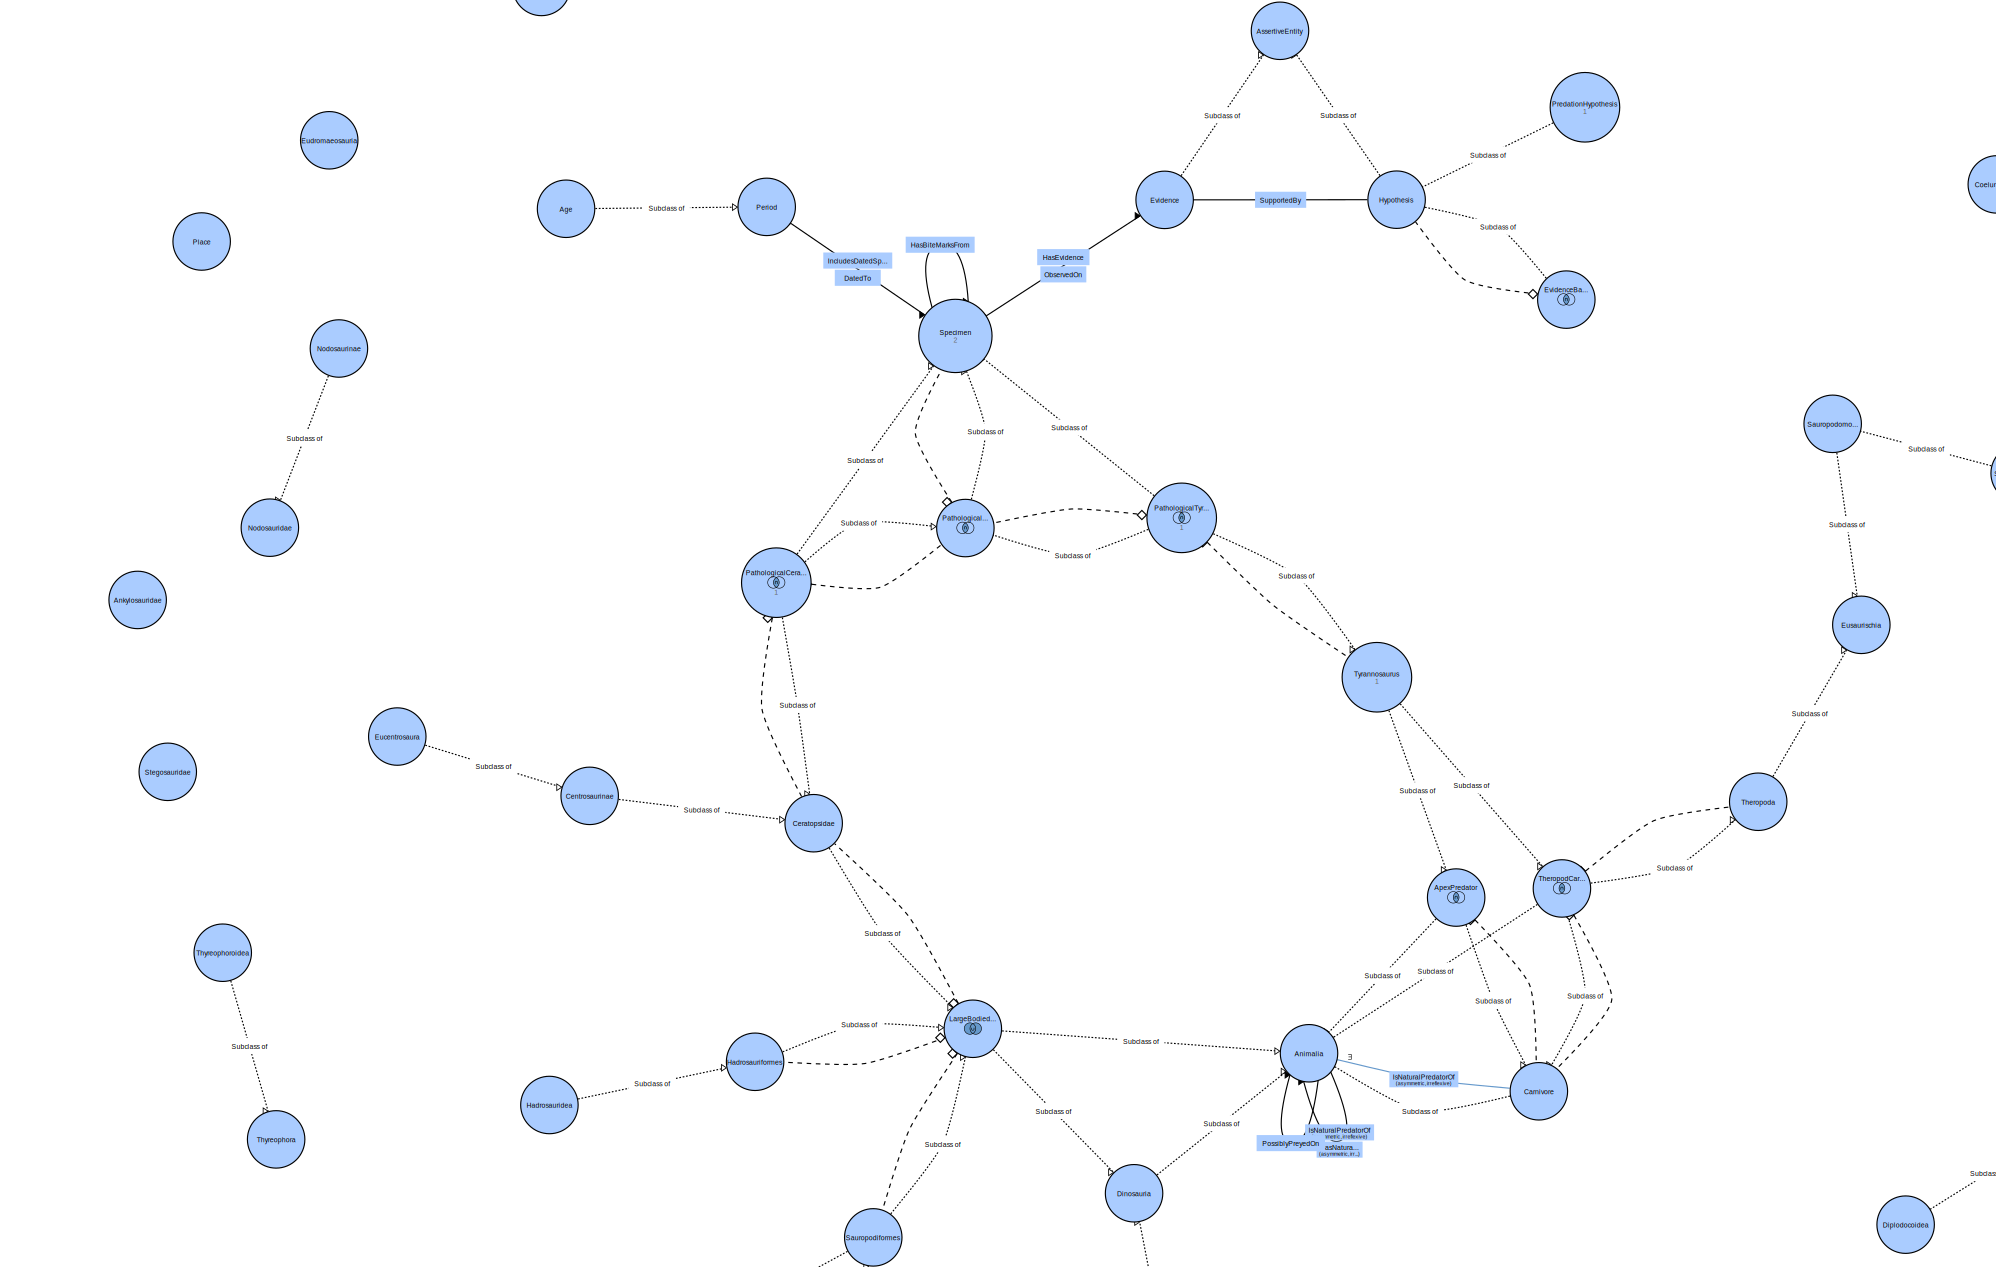
\includegraphics[width=150mm]{figures/animalia_specimen_4_degrees_filter.png}
		\caption{Приближение на свързаната компонента (слой) на онтологията с център на тежестта концепция за царство животни и надразред динозаври. За по-голям и интерактивен вариант отворете предоставения в архива файл animalia\_specimen\_4\_degrees\_filter.svg с предпочитан от вас браузър.}
	\end{figure}
	
	% trim=left bottom right top
	%\begin{figure}[h]
	%	\centering
	%	\includegraphics[width=0.8\textwidth, trim=0mm 16cm 0mm 2cm, clip]{dinosaur_onto.pdf}
	%	\caption{Онтология на разред динозаври}
	%	\label{fig:ontology_webvowl}
	%\end{figure}
	
	\newpage
	
	\section{Планиране и бъдещо развитие}\label{sec:future}
	
	Към базата от знания (онтологията) могат да бъдат добавени множество от известните на науката специмени, в момента за простота са илюстрирани само два индивида, тъй като те се нуждаят от още много индивиди, чрез които да бъдат обвързани. Не всички родове динозаври присъстват като листа в таксономията от концепции на надразред динозаври - за простата са въведени най-често по два рода, а в някой по-редки случаи дори по един. Добавянето на всички родове е трудоемка задача, но изпълнима от учените, като нейното изпълнение не би нарушило текущото функциониране на системата. Освен това вече съществуващи специмени биха могли с лекота да се класифицират към новодобавени или вече съществуващи родове, отново без нарушение на базата от знания.
	\newline\newline
	След това, към онтологията могат да бъдат добавени множество от неатомарни концепти, тъй като в момента са дефинирани прости такива, поради малкото количество налични тестови индивиди. Добавянето им би позволило базата от знания да извежда по-голям брой изводи, които генерализират поведения и открития и позволяват на учените да изпълняват DL заявки към базата от знанията. Освен това, след като населят онтологията с индивиди, попълвайки техните данни базирани на измервания от открития, те биха могли да конструират SPARQL заявки и да извличат интересни за науката палеонтология резултати.
	\newline\newline
	На последно място, не и по важност, голяма част от класовете могат да се обогатят с повече нужни данни и свойства, тъй като текущата база от знания набляга основно върху специмените и таксономията, като в случая на таксономията има потенциал да бъде доразвита по такъв начин, че да позволява автоматична видова класификация.
	
	\newpage
	
	\begin{thebibliography}{999}
		
		\bibitem{owlready2}
		\href{https://owlready2.readthedocs.io/en/latest/}{Owlready2}
		
		\bibitem{owl-guide}
		\href{https://www.w3.org/TR/owl-guide/}{OWL Web Ontology Language Guide}
		
		\bibitem{geol-104-dinosaurs}
		\href{https://www.geol.umd.edu/%7Etholtz/G104/lectures/104dinorise.html}{GEOL 104 Dinosaurs: A Natural History}
		
		\bibitem{ornithischia}
		\href{https://en.wikipedia.org/wiki/Ornithischia}{Ornithischia}
		
		\bibitem{thyreophora}
		\href{https://en.wikipedia.org/wiki/Thyreophora}{Thyreophora}
		
		\bibitem{cerapoda}
		\href{https://en.wikipedia.org/wiki/Cerapoda}{Cerapoda}
		
		\bibitem{saurischia}
		\href{https://en.wikipedia.org/wiki/Saurischia}{Saurischia}
		
		\bibitem{theropoda}
		\href{https://en.wikipedia.org/wiki/Theropoda}{Theropoda}
		
		\bibitem{sauropoda}
		\href{https://en.wikipedia.org/wiki/Sauropoda}{Sauropoda}
		
		
	\end{thebibliography}
	
\end{document}
